\chapter{Gravitação}


{\bf Problema 1} Um satélite deve ser lançado em uma órbita circular ao redor da Terra de modo que orbite o planeta uma vez a cada $T$ segundos.
(a) Mostre que a altitude h acima da superfície da Terra que o satélite deve ter é
$$h = \left( \frac{GMT^2}{4\pi^2}\right)^{\frac{1}{3}} - R$$,
onde $G = 6.67 \times 10^{-11} m^3 kg^{-1}s^{-2}$ é a constante gravitacional de Newton, $M = 5.97 \times 10^{24} kg$ é a massa da Terra e $R = 6371 km$ é o seu raio.
b) Escreva um programa que peça ao usuário para inserir o valor desejado de $T$ e então calcule e imprima a altitude correta em metros.
c) Use seu programa para calcular as altitudes dos satélites que orbitam a Terra uma vez
por dia (a chamada órbita ``geossíncrona''), uma vez a cada 90 minutos e uma vez a cada
45 minutos. O que você conclui do último desses cálculos?
d) Tecnicamente um satélite geossíncrono é aquele que orbita a Terra uma vez por dia sideral dia, que é 23,93 horas, não 24 horas. Por que é isso? E quanta diferença
fará à altitude do satélite?

\begin{lstlisting}[language=Python, frame=lines,basicstyle=\footnotesize, caption={Altitude de um Satélite}, label={lst:Satelite}]
from math import pi

# parametros e constantes kg, m, s
G = 6.67*10**(-11) 
M = 5.97*10**(24) 
R = 6371*10**3

#input
unit=input('Qual a unidade utilizada (dias, horas, minutos, segundos)?')
period = float(input('Qual o periodo?'))
if not unit in ['dias', 'horas', 'minutos', 'segundos']:
    print('Unidade nao Reconhecida')
elif unit == 'dias':
    period = 24*60*60*period
elif unit == 'horas':
    period = 60*60*period
elif unit == 'minutos':
    period = 60*period

h = (G*M*period**2/(4*pi**2))**(1/3)-R
print(h, ' m')
\end{lstlisting}


\section{Terceira Lei de Kepler}

Arquivo {\tt jupyter-moons.csv} disponivel no github.
\begin{lstlisting}[language=Python, frame=lines,basicstyle=\footnotesize, caption={Lus de Jupyter e A terceira Lei de Kepler}, label={lst:jup-k-3law}]
import matplotlib.pyplot as plt
import pandas as pd
import numpy as np
import matplotlib.colors as mcolors

plt.rcParams["figure.figsize"] = (12,12)

df = pd.read_csv('jupyter-moons.csv')
fit = np.polyfit(np.log(np.absolute(df.Orbital_period)), np.log(df.Semi_major_axis), 1)
p_fit = np.poly1d(fit)
log_t = np.linspace(-1.5,7.2)

#Color dictionary for groups
types=list(set(df.Group))
colors = list(list(mcolors.CSS4_COLORS))   
color_dict={types[i]: colors[i+10] for i in range(len(types))}
color_map = [color_dict[i] for i in list(df.Group)]

plt.scatter(np.log(np.absolute(df.Orbital_period)),np.log(df.Semi_major_axis),c = color_map, s=df.log_mass)
plt.ylabel('log Semi-major axis (km)')
plt.xlabel('log Orbital Period (days)')
plt.title('Jupyter`s Moons')
plt.grid()
markers = [plt.Line2D([0,0],[0,0],color=color, marker='o', linestyle='') for color in color_dict.values()]
plt.legend(markers, color_dict.keys(), numpoints=1, title='Moon Group')
plt.plot(log_t, p_fit(log_t), linestyle='dashed')
plt.annotate(p_fit, (3.75,15), rotation=45)
plt.show()
\end{lstlisting}

O resultado deve ser semelhante ao abaixo

\begin{figure}[h!]
\centering
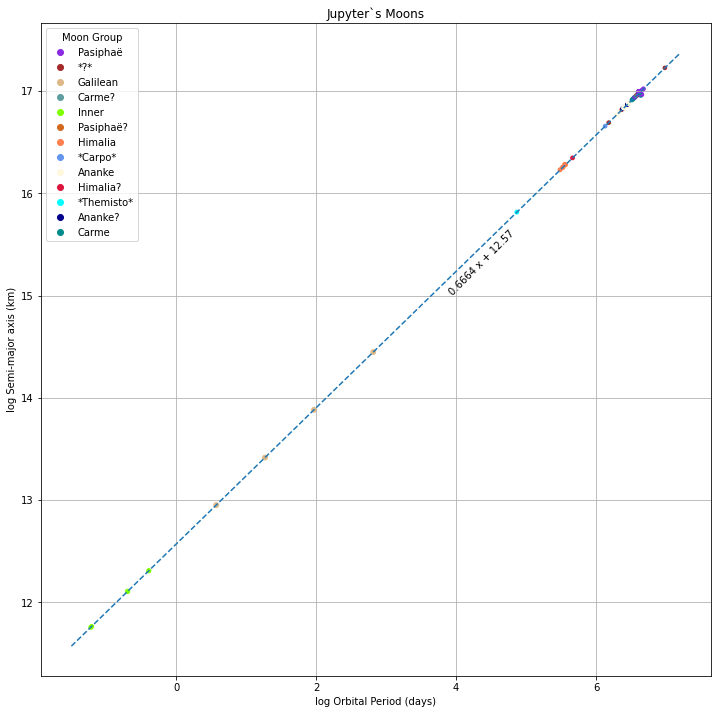
\includegraphics[scale=0.5]{Images/jupyter-moons.png}
\caption{Gráfico dos dados orbitais das luas de Júpiter obtidos do arquivo {\tt jupyter-moons.csv}}\label{fig:Jupyter-moons}
\end{figure}

Problemas do Haliday Capítulo 13

1. Larry Niven wrote a series of science fiction books about
Ringworld, an inhabited, manufactured ring of metal that cir-
cled a star. Consider a uniform ring of material with total
mass M and radius R. Assume that the ring is infinitesimally
thin. In terms of G, M, and R, (a) calculate the gravitational
potential energy at a point r = R /2 in the plane of the ring,
and (b) calculate the magnitude and direction of the force of
gravity on a 1-kg mass located at that same point. (c) Repeat
(a) and (b) for a point r = 3R /2 in the plane of the ring. (See
“Bound Orbits with Positive Energy,” by J. West, S. Das-
sanayake, and A. Daniel, American Journal of Physics, Janu-
ary 1998, p. 25.)
2. Repeat Problem 23 for 19 particles, 29 particles, 39 particles,
and so on up to 99 particles. Plot the results on a graph of
number of particles versus rotational period. Does the result
converge to a limit as the number of particles becomes infi-
nite? If so, what is that limit? Can the problem be solved ana-
lytically?

Problema de Kepler 2 corpos

\textcolor{red}{Ainda possui um erro}

\begin{lstlisting}[language=Python, frame=lines,basicstyle=\footnotesize, caption={Orbitas: Problema de Kepler para 2 Corpos}, label={lst:2body-kepler}]
import numpy as np
import matplotlib.pyplot as plt

#Parameters
GM = 1
pi = np.pi

#Simulation Parameters
dt = .001 # time step
T  = 10 # total simulation time, T/dt will give the total number of steps

# Deal with polar coordinates
def polar_coord(x, y):
    r = np.sqrt(x**2+y**2)
    if x == 0:
        theta = np.sign(y)*pi/2
    else:
        theta = np.arctan(y/x)
    return r, theta

def polar_vector(x,y,vx,vy):
    r, theta = polar_coord(x,y)
    hatr = np.array([np.cos(theta), np.sin(theta)])
    hattheta = np.array([-np.sin(theta), np.cos(theta)])
    vpolar = np.linalg.solve([hatr, hattheta], [vx, vy])
    vr, vtheta = vpolar[0], vpolar[1]
    return vr, vtheta

class Planet: # Create Class Planet
    def __init__(self, x, y, vx, vy, mass):
        self.mass = mass
        r0 , theta0 = polar_coord(x,y)
        self.r, self.theta = r0, theta0
        self.rtraj = [self.r]
        self.thetatraj = [self.theta]
        self.vr, self.vtheta = polar_vector(x, y, vx, vy)
        self.L = mass*r0**2*self.vtheta
        self.energy = (1/2)*mass*(vx**2+vy**2)-GM*mass/r0
    
    def move(self): # Move Planet
        self.r += dt*self.vr #Up date r positions
        self.theta += dt*self.vtheta #Up date Y positions
        #Update r trajectory
        self.rtraj = np.append(self.rtraj, self.r)
        self.thetatraj = np.append(self.thetatraj, self.theta) #Up date theta trajectory
        potential_f = - GM*self.mass/self.r**2
        centrifugal_f = self.L**2/(self.mass*self.r**3)
        f_eff = potential_f +  centrifugal_f
        self.vr +=  dt*f_eff/self.mass
        self.vtheta = self.L/(self.mass*self.r**2)

# Create a planet
planet = Planet(1,0,0.1,1,1)
t = 0
while planet.theta <= 2*pi: 
    planet.move()
    t += dt
    if t >= 10**9:
        break
    else:
        continue

r_max = np.amax(planet.rtraj)
r_min = np.amin(planet.rtraj)
print('Periodo orbital =', t)
print('Afelio =', r_max)
print('Perielio =', r_min)
print('excentricidade=', (r_max - r_min)/(r_max+r_min))

#Plot Orbit

fig, ax = plt.subplots(subplot_kw={'projection': 'polar'})
ax.plot(planet.thetatraj, planet.rtraj)
ax.plot(planet.thetatraj[0], planet.rtraj[0],'ro', markersize=8)
ax.plot(planet.thetatraj[-1], planet.rtraj[-1],'b+', markersize=8)
ax.set_rmax(1.1*r_max)
ax.grid(True)
ax.set_title("Motion of the Planet", va='bottom')
plt.show()

\end{lstlisting}

Problema de Kepler Sol-Terra-Lua
ver \\
\href{URL}{https://drive.google.com/file/d/1maO81Tll58t7KZXXaIZzalZ3JtpMEsio/view}
